\documentclass[a4paper, 11pt]{report}
\usepackage{graphicx} % Required for inserting images
\usepackage{amsfonts}
\usepackage{amssymb}
\usepackage{tikz,lipsum,lmodern}
\usepackage[most]{tcolorbox}
\usepackage{pgfplots}
\usepackage{tabularx}
\usepackage{stmaryrd}
\usepackage{tikz} 
\usepackage{imakeidx}
\usepackage{hyperref}
\usepackage{titlesec}
\usepackage{enumitem}

\usetikzlibrary{calc}
\makeindex[columns=3, title=Alphabetical Index, intoc]
\hypersetup{
    colorlinks=true,
    linkcolor=blue!50!green!70!black,
    filecolor=magenta,      
    urlcolor=blue,
    pdftitle={Max flows in O(nm) time, or better},
    pdfpagemode=FullScreen,
    }

\newcommand*{\QED}{\null\nobreak\hfill\ensuremath{\square}}%
\newcommand*{\proof}{\textit{proof}:\\}
\newcommand*{\mb}[1]{\mathbb{#1}}
\newcommand*{\mc}[1]{\mathcal{#1}}

\definecolor{bananamania}{rgb}{0.98, 0.91, 0.71}
\definecolor{amaranth}{rgb}{0.9, 0.17, 0.31}
\definecolor{amethyst}{rgb}{0.6, 0.4, 0.8}
\definecolor{darktangerine}{rgb}{1.0, 0.66, 0.07}
\definecolor{cerise}{rgb}{0.87, 0.19, 0.39}
\definecolor{babyblue}{rgb}{0.54, 0.81, 0.94}
\definecolor{brightgreen}{rgb}{0.4, 1.0, 0.0}

\newtcbtheorem[auto counter]{theo}%
  {Theorem}{fonttitle=\bfseries,
    colback=white!5!white,colframe=amaranth}{theo}

\newtcbtheorem[auto counter,number within=section]{corollary}%
    {Corollary}{fonttitle=\bfseries,
      colback=white,colframe=cerise}{corollary}

\newtcbtheorem[auto counter]{definition}%
    {Definition}{fonttitle=\bfseries,
    colback=white!5!white,colframe=teal!60!green}{definition}

\newtcbtheorem[auto counter]{lemma}%
    {Lemma}{fonttitle=\bfseries,
    colback=white!5!white,colframe=amethyst}{lemma}

\newtcbtheorem[auto counter]{obs}%
    {Observation}{fonttitle=\bfseries,
    colback=white!5!white,colframe=darktangerine}{obs}

\newtcbtheorem[auto counter]{proposition}%
    {Proposition}{fonttitle=\bfseries,
    colback=white!5!white,colframe=magenta}{proposition}

\newtcbtheorem[auto counter]{algo}%
    {Algorithm}{fonttitle=\bfseries,
    colback=white,colframe=green!50!black!60!blue}{algo}

\newtcbtheorem[auto counter]{remark}%
    {Remark}{fonttitle=\bfseries,
    colback=white,colframe=bananamania,coltitle = brown!45!black}{remark}

\newtcbtheorem[auto counter]{example}%
    {Example}{fonttitle=\bfseries,
    colback=white,colframe=babyblue!70!white,coltitle = blue!45!black}{example}

\titlespacing*{\chapter}{0pt}{-20pt}{20pt} % Riduce lo spazio prima del titolo del capitolo
\titleformat{\chapter}[display]
  {\normalfont\Large\bfseries} % Stile del titolo
  {\chaptername\ \thechapter}{10pt}{\huge}

\title{Max flows in O(nm) time, or better\\
\large Appunti per la tesi}

\author{Armando Coppola}
\date{\today}



\begin{document}
\maketitle
\newpage
\tableofcontents
\newpage
\section*{Introduzione}
Ciò che segue è una relazione che ha lo scopo di analizzare la soluzione proposta nell'algoritmo di Prim per il calcolo del \textbf{max flow in un Network}.
Dato che per comprendere a pieno il suo funzionamento è necessario conoscere anche alcuni algoritmi precedenti, anche questi vengono spiegati nella relazione. 
Gli algoritmi sono presentati in ordine cronologico a partire dall'algoritmo di Dinics, continuando con Goldberg-Rao e giungendo alla soluzione più recente e efficace di Prim.
Prima di iniziare con le soluzioni però, è presente un capitolo che spiega alcune nozioni preliminari sulla teoria dei grafi necessarie per comprendere il funzionamento delle soluzioni.

\chapter{Preliminary notions}
\section{Network e flow}
\begin{definition}{Network}{}
    Definiamo un Network come una struttura composta da un grafo $G = (N,E)$ tale che:\begin{itemize}
        \item N = insieme dei nodi 
        \item E = $\{(i,g)\land i,g \in N \}$ insieme degli archi 
        \item $n$ = $|N|$
        \item $m$ = $|E|$
    \end{itemize}
    e composta da una funzione $u: E \rightarrow \mathbb{N}^+\cup \{+\infty\}$ che denota la capacità di ogni arco.
    \[u(i,j) = \text{capacità dell'arco } (i,j)\]
    \begin{center}
        \textit{indicheremo di seguito la capacità $u(i,j)$ con l'abbreviazione $u_{ij}$}
    \end{center}
\end{definition}
In ogni Network esistono due nodi speciali, s \textit{source} e t \textit{sink}. lo scopo di un Network è inviare flusso dal nodo s al nodo t.
\begin{figure}
    \centering
    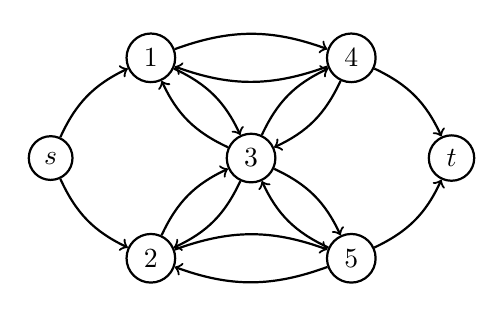
\begin{tikzpicture}[node distance={18mm}, thick, main/.style = {draw, circle}] 
        \node[main] (0) {$s$}; 
        \node[main] (1) [above right of=0] {$1$};
        \node[main] (2) [below right of= 0] {$2$};
        \node[main] (3) [above right of = 2] {$3$};
        \node[main] (4) [above right of=3] {$4$};
        \node[main] (5) [below right of=3] {$5$};
        \node[main] (6) [below right of=4] {$t$};
        
    
    
        \draw[->] (0) to [bend left = 20] (1);

    
        \draw[->] (0) to [bend right = 20] (2);

    
        \draw[->] (2) to [bend left= 20] (3);
        \draw[->] (3) to [bend left= 20] (2);
    
        \draw[->] (1) to [bend left= 20] (3);
        \draw[->] (3) to [bend left= 20] (1);

        \draw[->] (4) to [bend left= 20] (3);
        \draw[->] (3) to [bend left= 20] (4);

        \draw[->] (5) to [bend left= 20] (3);
        \draw[->] (3) to [bend left= 20] (5);

        \draw[->] (1) to [bend left= 20] (4);
        \draw[->] (4) to [bend left= 20] (1);


        \draw[->] (4) to [bend left= 20] (6);

        \draw[->] (5) to [bend left= 20] (2);
        \draw[->] (2) to [bend left= 20] (5);

        \draw[->] (5) to [bend right= 20] (6);

    
    \end{tikzpicture} 
    \caption{Esempio classico di un Network}
\end{figure}



\begin{definition}{$U_{min},\ U_{max}$}{}
    In ogni nodo definiamo come:
    \begin{itemize}
        \item $U_{min}$: la più piccola capacità non zero associata ad un arco:
        \[U_{min} = u_{ij} | (i,j) \in E\ \land\ u_{ij} > 0\ \land\ \nexists (k,l) \in E : 0<u_{kl}<u_{ij}\]
        \item $U_{max}$: la più grande capacità finita 
        \[U_{max} = u_{ij}| (i,j) \in E\land u_{ij} \not = + \infty\ \land \]
        \[\nexists (k,l) \in E : u_{ij}< u_{jl} < +\infty \]
    \end{itemize}
\end{definition}
distingiuiamo gli archi del Network in:\\
\textbf{External Arcs} := $\{(x,y) | (x,y)\in E \land (x = s \lor y = t)\}$\\
\textbf{Internal Arcs} := $\{(x,y) | (x,y)\in E \land x \not = s \land y \not = t\}$ ovvero $E \setminus External\ Arcs$\\
\\
Assumeremo che per ogni $(i,j)$ internal arc allora esiste $(j,i) \in E$.\\ In oltre per ogni internal node $i$ esiste $(s,i) \in E \land (i,t) \in E$ eventualmente con capacità 0
\begin{obs}{}{}
    Il nodo $s$ non ha archi entranti come il nodo $t$ non ha archi uscenti
\end{obs}

\begin{definition}{Flow}{}
    Definiamo come con la funzione $f: E \rightarrow\mathbb{R}_+ \cup \{0\}$ che soddisfa la $flow\ conservation$
    \[\sum_{j:(i,j) \in E} f_{ij} - \sum_{j:(j,i) \in E}f_{ji} = 0 \quad \forall i \in N\setminus\{s,t\}\]
\end{definition}

Un \textit{flow} si dice \textit{feasible} se $\forall (i,j) \in E,\ f_{ij} \le u_{ij}$(\textit{capacity constraints}).\\
Il valore del flow è dato dalla somma del flow degli archi uscenti da s o entranti in t.  
\begin{definition}{residual capacity}{}
    La capacità residua da $i \rightarrow j$ indica la quantita di flusso che si può ancora immettere dal nodo i al nodo j
    \[r_{ij} = u_{ij} + f_{ji} - f_{ij}\]    
    quando parleremo di capacità residue secondo diversi flow potremmo usare anche la notazione:
    \[u_f(i,j)\]
    che indica proprio la capacità residuo di un arco attraversato dal flow $f$
\end{definition}

\begin{definition}{Residual Graph}{}
    Dato un Network $\mc{N}$ e un un flusso $f$ definito sul grafo possiamo definire il grafo residuo come 
    \[G_f := (N(\mc{N}), \{(i,j) | (i,j)\in E(\mc{N}) \land r_{ij} > 0\})\]
    
\end{definition}

\begin{definition}{s-t Cut}{}
    Definiamo come $s-t\ Cut$ la partizione di G in due sottoinsiemi (S,T) tali che:
    \begin{enumerate}
        \item $s \in S$
        \item $t \in T$
        \item $S \cap T = \varnothing$
        \item $S \cup T = N$
    \end{enumerate}
    
    La \textit{capacità} del Cut è definita come:
    \[u(S,T) = \sum_{i\in S\land j\in T} u_{ij}\]
    Il \textit{residuo} del taglio: è definito come:
    \[r(S,T) = \sum_{i\in S\land j\in T} r_{ij}\]
\end{definition}

\begin{lemma}{Max residual flow min residual cut}{}
    Dato un grafo residuo $G_f$ e un cut (S,T) allora $r(S,T)$ rappresenta l'upper bound dell flusso da $s \rightarrow t$.
    In particolare, il massimo incremento di flow rispetto ad $r$ è la capacita residua minore di un s-t cut.  
\end{lemma}
\textit{dimostrazione omessa}\\
Il lemma riporta che il problema di trovare il flusso massimo su un Network è \textbf{duale} a quello di trovare un taglio di capacità minima sullo stesso network in quanto questo rappresenterà il collo di bottiglia che fa da upper bound all'aumento di flusso.

\begin{definition}{Anti-symetric subset}{}
    Dato $E(j)$ l'insieme degli archi adiacenti con j definiamo come \textit{Anti-symetric} subset 
    \[E'(j) :=\{(x,y)|(x,y)\in E(j) \land (x,y) \in E'(j) \iff (y,x) \not\in E'(j)\}\] 
\end{definition}
\textbf{Esempio:}\\
\begin{center}
    
\begin{tabular}{cc|cc}
    $E(j)  $&\qquad &\qquad& $E'(j)  $\\
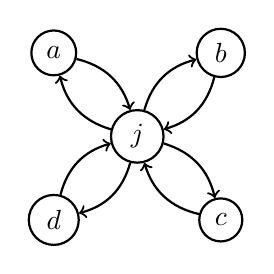
\begin{tikzpicture}[node distance={15mm}, thick, main/.style = {draw, circle}] 
    \node[main] (1) {$j$}; 
    \node[main] (2) [above right of=1] {$b$};
    \node[main] (3) [below right of=1] {$c$};
    \node[main] (4) [above left of=1] {$a$};
    \node[main] (5) [below left of=1] {$d$};


    \draw[->] (2) to [bend left] (1);
    \draw[->] (1) to [bend left] (2);

    \draw[->] (3) to [bend left] (1);
    \draw[->] (1) to [bend left] (3);

    \draw[->] (4) to [bend left] (1);
    \draw[->] (1) to [bend left] (4);

    \draw[->] (5) to [bend left] (1);
    \draw[->] (1) to [bend left] (5);

\end{tikzpicture} 
&&
&
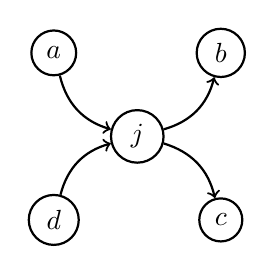
\begin{tikzpicture}[node distance={15mm}, thick, main/.style = {draw, circle}] 
    \node[main] (1) {$j$}; 
    \node[main] (2) [above right of=1] {$b$};
    \node[main] (3) [below right of=1] {$c$};
    \node[main] (4) [above left of=1] {$a$};
    \node[main] (5) [below left of=1] {$d$};



    \draw[->] (1) to [bend right] (2);


    \draw[->] (1) to [bend left] (3);

    \draw[->] (4) to [bend right] (1);


    \draw[->] (5) to [bend left] (1);


\end{tikzpicture} 
\end{tabular}
\end{center}
\begin{lemma}{Anti-symmetriy lemma}{}
    Dato $E'(j)$ un anti-symmetric subset di $E(j)$ e un flusso $f$ su $G$ con $r = r[f]$ allora:
    \[\sum_{(i,j)\in E'(j)}r_{ij} - \sum_{(j,i)\in E'(j)}r_{ji} = \sum_{(i,j)\in E'(j)}u_{ij} - \sum_{(j,i)\in E'(j)}u_{ji} \]
\end{lemma}
\begin{proof}
    \[\sum_{(i,j)\in E'(j)}r_{ij} - \sum_{(j,i)\in E'(j)}r_{ji} -\sum_{(i,j)\in E'(j)}u_{ij} + \sum_{(j,i)\in E'(j)}u_{ji}= 0 \implies\]
    \[\sum_{(i,j)\in E'(j)}(u_{ij}-r_{ij}) + \sum_{(j,i)\in E'(j)}(u_{ji}-r_{ji}) = 0 \]
    dato che $r_{ij} = u_{ij} - f_{ji} + f_{ij} \implies u_{ij} -r_{ij} = f_{ji}- f_{ij}$ 
    \[\sum_{(i,j)\in E'(j)}(f_{ji}-f_{ij}) + \sum_{(j,i)\in E'(j)}(f_{ij}-f_{ji}) = \sum_{(i,j)\in E(j)}(f_{ji}-f_{ij}) = 0\]
    ovvero il vincolo di \textit{conservazione del flow}
    \QED
\end{proof}
\section{Decomposition e transfering del flow}

\begin{definition}{Flow decomposiiton}{}
    Dato $f$ un $s-t$ flow su $N$, definiamo  \textit{flow-decomposition}, una collezione di $s-t$ path diretti
    \[P_1, ..., P_s\quad \phi_1,..., \phi_s\]
    tale che: \begin{enumerate}
        \item $\forall (u,v) \in P_i, f(u,v)> 0$
        \item $f(P_i) = \phi_i\ \forall i, \in [1,s]$
        \item $ val(f) = \sum_{i = 1}^s \phi_i$
    \end{enumerate}


\end{definition}
Un \textbf{osservazione} intuitiva è che il massimo numero di decomposizioni di un $flow$ è $m$.\\
\begin{center}
    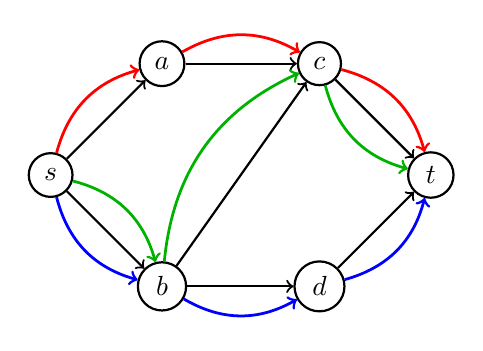
\begin{tikzpicture}[node distance={20mm}, thick , main/.style = {draw, circle}] 
    \node[main] (1) {$s$}; 
    \node[main] (2) [above right of=1] {$a$};
    \node[main] (3) [below right of=1] {$b$};
    \node[main] (4) [right of=2] {$c$};
    \node[main] (5) [right of=3] {$d$};
    \node[main] (6) [above right of=5] {$t$};
    %Admissible
    \draw[->] (1) to (2);
    \draw[->] (1) to (3);
    \draw[->] (3) to (5);
    \draw[->] (2) to (4);
    \draw[->] (5) to (6);
    \draw[->] (4) to (6);
    \draw[->] (3) to (4);
    
    %paths
    \draw[->,line width=1 pt] (1)[red, bend left] to (2);
    \draw[->,line width=1 pt] (2)[red, bend left] to (4);
    \draw[->,line width=1 pt] (4)[red, bend left] to (6);

    \draw[->,line width=1 pt] (1)[blue, bend right] to (3);
    \draw[->,line width=1 pt] (3)[blue, bend right] to (5);
    \draw[->,line width=1 pt] (5)[blue, bend right] to (6);

    \draw[->,line width=1 pt] (1)[green!70!black, bend left] to (3);
    \draw[->,line width=1 pt] (3)[green!70!black, bend left] to (4);
    \draw[->,line width=1 pt] (4)[green!70!black, bend right] to (6);

\end{tikzpicture} \\
Esempio di flow decomposto
\end{center}
Da questo grafo possiamo notare che (capacità permettendo ovviamente), un feasible flow da $s \rightarrow t$ può essere decomposto come il percorsi con \textbf{almeno un arco 
differente} che lo compongono. In particolare notiamo nel grafo:
\begin{itemize}
    \item  in \textbf{nero} il grafo del network
    \item in \textbf{\color{red}{rosso}}, \textbf{\color{green!70!black}{verde}} e \textbf{\color{blue}{blu}} tre differenti $paths$ da $s\rightarrow t$
\end{itemize}
\newpage
Un'altro passaggio fondamentale da comprendere per la risoluzione del problema il trasferimento di capacità.
\begin{definition}{Tranfer}{}
    Dato un arco $(i,j) \in E$ e un $path\ P\ i\rightarrow j$ con $|P|\ge 2$, \textbf{trasferire} $\delta$ unita di capacità da $P$ a $(i,j)$
    significa ridurre $\forall (k,l) \in P$ $u_{kl}$ di $\delta$ unità e aggiungere $\delta$ unità a $u_{ij}$ 
\end{definition}
\begin{lemma}{capacity tranfer lemma}{}
    Sia $P$ un $path$ in $G$ da $i$ a $j$ e sia $(S,T)$ un taglio. Sia $u'$ la capacità dell'arco $(i,j)$ ottenuta trasferendo $\delta$ capacità dal path $P$. Allora è vero che
    \[u'(S,T) \le u(S,T)\] 
\end{lemma}
\begin{proof}
    La dimostrazione è banale se $i,j \in S \lor i,j \in T$ dato che $u'(P) \le u(P) \implies u'(S,T)\le u(S,T)$.\\
    Mentre invece se $i\in S \land j \in T$, se consideriamo $k \in P$ il primo nodo di $P$ in $T$ e $l \in P$ il nodo subito precedente a $k$, possiamo stimare 
    \[u'(S,T)-u(S,T)\le (u'_{kl}+u'_{ij})- (u_{kl}+u_{ij}) = -\delta + \delta = 0\]\QED
\end{proof}


\[\begin{tabular}{c|c}
    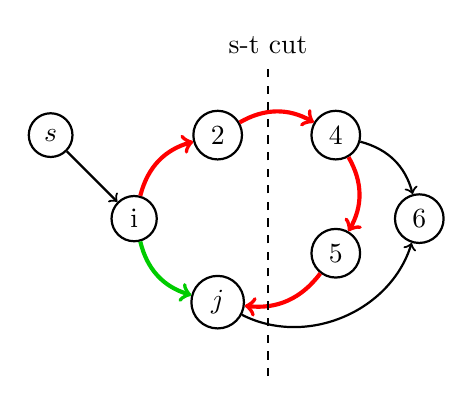
\begin{tikzpicture}[node distance={15mm}, thick , main/.style = {draw, circle}] 
    % Disegna i nodi del grafo
    
    \node[main] (1) {i};
    \node[main] (0) [above left of = 1] {$s$};
    \node[main] (2) [above right of=1] {$2$};
    \node[main] (3) [below right of=1] {$j$};
    \node[main] (4) [right of=2] {$4$};
    \node[main] (6) [below right of=4] {$6$};
    \node[main] (5) [below of=4] {$5$};
    % Disegna gli archi orientati
    \draw[->] (0) to (1);
    \draw[->,line width=1.5 pt] (1)[red, bend left] to (2);
    \draw[->,line width=1.5 pt] (1)[green!80!black, bend right] to (3);
    \draw[->,line width=1.5 pt] (2)[red, bend left] to (4);
    \draw[->,line width=1.5 pt] (4)[red,bend left] to (5);
    \draw[->] (4)[bend left] to (6);
    \draw[->] (3)[bend right = 50] to (6);
    \draw[->,line width=1.5 pt] (5)[red,bend left] to (3);

    % Aggiungi una linea tratteggiata per dividere il grafo in due
    \draw[dashed] (1.7,-2) -- (1.7,2);
    \node at (1.7,2.2) {s-t\ cut};

\end{tikzpicture}& 
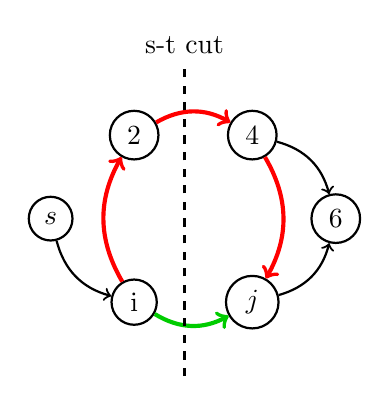
\begin{tikzpicture}[node distance={15mm}, thick , main/.style = {draw, circle}] 
    % Disegna i nodi del grafo
    
    
    \node[main] (0) {$s$};
    \node[main] (1) [below right of = 0] {i};
    \node[main] (2) [above right of=0] {$2$};
    \node[main] (4) [right of=2] {$4$};
    \node[main] (6) [below right of=4] {$6$};
    \node[main] (3) [below left of=6] {$j$};
    % Disegna gli archi orientati
    \draw[->] (0)[bend right] to (1);
    \draw[->,line width=1.5 pt] (1)[red, bend left] to (2);
    \draw[->,line width=1.5 pt] (1)[green!80!black, bend right] to (3);
    \draw[->,line width=1.5 pt] (2)[red, bend left] to (4);
    \draw[->,line width=1.5 pt] (4)[red, bend left] to (3);
    
    \draw[->] (4)[bend left] to (6);
    \draw[->] (3)[bend right] to (6);


    % Aggiungi una linea tratteggiata per dividere il grafo in due
    \draw[dashed] (1.7,-2) -- (1.7,2);
    \node at (1.7,2.2) {s-t\ cut};

\end{tikzpicture}\\
    \multicolumn{2}{c}{in {\color{red}{rosso}} il path P, in {\color{green!80!black}{verde}} l'arco (i,j)}
 


\end{tabular}\]

Possiamo dire in generale quindi che trasferire capacità non aumenta il max flow instradabile in un network.

\newpage
\section{Distance based}
\begin{definition}[label = VDL]{Valid distance labeling}{}
    Siano $N = (G,u)$ un Network, $f$ un feasible flow su $N$ e $l((u,v))$ una funzione che sancisce \textit{lunghezza} di ogni arco in $G$.\\
    La funzione di \textbf{distanza} $d: N(G) \rightarrow \mathbb{N}$ rispetto al \textbf{residual graph}
    $G(f)$  si dice \textbf{valida} se soddisfa le seguenti proprietà:
    \begin{enumerate}
        \item $d(t) = 0$
        \item $d(i) \le d(j) + l((i,j))$
    \end{enumerate}
\end{definition}
\textbf{Nota:} Se non diversamente specificato, una funzione $l((u,v))$ associa ad ogni arco del grafo la lunghezza $1$,
 tuttavia può anche essere specificata, come nel caso dell'algorimo di \textbf{Goldberg-Rao}(che segue),
una funzione di lunghezza diversa. 
\begin{obs}{Valid distance label property}{}
    Una valid distance label, $d$, preserva le seguenti proprietà:
    \begin{enumerate}
        \item $d(i)$ rappresenta il \textit{lower bound} della lunghezza dello shortest directed path da $i \rightarrow t$
        nel resiudual graph
        \item $d(s) \ge n \implies \nexists p\ path \in G(f) | p = s \rightarrow t $ %va spegato meglio la notazione di grafo residuo e di path
    \end{enumerate}
    
\end{obs}
Un altro significato (forse l'idea di fondo) della distance labeling sta in \[\neg (d(v) > d(w) + l(v,w))\]
Ovvero, se $w,v \in N \land (v,w) \in E$ allora la distanza di $v$ non può mai superare la distanza di $w$ più la lunghezza tra i due nuovi, 
proprio per definizione di shortest path.

\begin{definition}[label = AdmissibleGraph]{Admissible graph}{}
    Siano $N = (G,u)$ un Network $N = (G,u)$ con un feasible flow $f$, $d: N(G(f)) \rightarrow \mathbb{N}$ valid distance label 
    e $l((u,v))$ una length function.
    un \textit{residual arc} si dice \textbf{Admissible arc} se soddisfa:
    \[d(v) = d(w) + l(v,w) \quad \forall (v,w) \in E(G(f))\]
    ovvero:
    \[d(v) > d(w) \lor (d(v) = d(w) \land l(v,w) = 0)\]
    
    $A(f,l,d)$ rappresenta l'\textbf{Admissible graph}, ovvero il grafo formato da tutti gli Admissible arc, rispetto alla distanza $d$ con lunghezze $l$ 
    sul resiudual graph dato dal flow $f$.
\end{definition}


\begin{obs}{}{}
    Sia $G(f)$ un grafo residuo, sia $B_s$ un'arborescenza data da una BFS sul grafo $G(f)$ dal nodo $s$ e sia $A$ l'\textit{admissible graph} allora
    \[E(B_s)\subsetneq E(A)\]
\end{obs}

\[
    \begin{array}{c|c|c}
        
    
    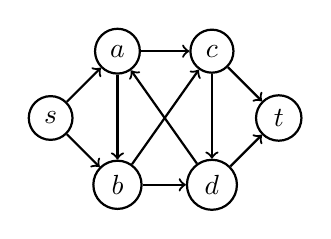
\begin{tikzpicture}[node distance={12mm}, thick , main/.style = {draw, circle}] 
    \node[main] (1) {$s$}; 
    \node[main] (2) [above right of=1] {$a$};
    \node[main] (3) [below right of=1] {$b$};
    \node[main] (4) [right of=2] {$c$};
    \node[main] (5) [right of=3] {$d$};
    \node[main] (6) [above right of=5] {$t$};
    %Admissible
    \draw[->] (1) to (2);
    \draw[->] (1) to (3);
    \draw[->] (3) to (5);
    \draw[->] (2) to (4);
    \draw[->] (5) to (6);
    \draw[->] (4) to (6);
    \draw[->] (3) to (4);
    \draw[->] (4) to (5);
    \draw[->] (5) to (2);
    \draw[->] (2) to (3);
\end{tikzpicture}  &
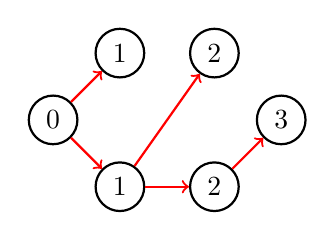
\begin{tikzpicture}[node distance={12mm}, thick , main/.style = {draw, circle}] 
    \node[main] (1) {$0$}; 
    \node[main] (2) [above right of=1] {$1$};
    \node[main] (3) [below right of=1] {$1$};
    \node[main] (4) [right of=2] {$2$};
    \node[main] (5) [right of=3] {$2$};
    \node[main] (6) [above right of=5] {$3$};
    %Admissible
    \draw[->, red] (1) to (2);
    \draw[->, red] (1) to (3);
    \draw[->, red] (3) to (5);
    \draw[->, red] (5) to (6);
    \draw[->, red] (3) to (4);
\end{tikzpicture} &
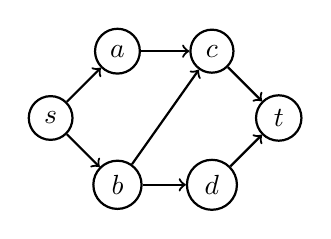
\begin{tikzpicture}[node distance={12mm}, thick , main/.style = {draw, circle}] 
    \node[main] (1) {$s$}; 
    \node[main] (2) [above right of=1] {$a$};
    \node[main] (3) [below right of=1] {$b$};
    \node[main] (4) [right of=2] {$c$};
    \node[main] (5) [right of=3] {$d$};
    \node[main] (6) [above right of=5] {$t$};
    %Admissible
    \draw[->] (1) to (2);
    \draw[->] (1) to (3);
    \draw[->] (3) to (5);
    \draw[->] (5) to (6);
    \draw[->] (3) to (4);
    \draw[->] (2) to (4);
    \draw[->] (4) to (6);
\end{tikzpicture} \\
\text{grafo originale}&\text{arborescenza} & \text{Admissible graph}
\end{array} 
\]
Ora che sono state definite le valid distance label, possiamo richiamare gli $s-t\ cut$ per definire i \textbf{canonical cuts}.
\begin{definition}[label = cancut]{Canonical cut}{}
    Dato un Network $\mc{N}$, e una distance label $d$ su $\mc{N}$, si definisce taglio canonico una partizione dei nodi del grafo 
    \[(S_k, T_k) =  (S_k:=\{v\in V(\mc{N}) | d(v) \ge k\},\ T_k := V(\mc{N})\setminus S_k)\]
\end{definition}
\newpage

\chapter{Past Algorithm}
\section{Dinic's Algorithm}
\label{dnc}
L'algoritmo segue l'\href{https://en.wikipedia.org/wiki/Edmonds%E2%80%93Karp_algorithm}{Edmonds-Karp} ma ragionando sul fatto che ogni volta che eseguo una BFS creo un albero di copertura con \underline{livelli} che indicano la distanza dal nodo di partenza.
quindi invece di eseguire una BFS e poi saturare solo uno dei percorsi minimi trovati, posso saturarli tutti prima di eseguire di nuovo una BFS.\\
Ogni volta che si esegue una BFS dalla \textit{source} si entra nella \textbf{blocking flow phase}.\\
\begin{definition}{Blocking flow}{}
    Per \textbf{blocking flow} si intende un flusso su un grafo (in questo caso il residuo del level graph) che satura almeno un arco per ogni possibile \textit{path} da $s\rightarrow t$.    
\end{definition}
\begin{obs}{Max flow $\implies$ blocking flow}{}
    Il max flow è un blocking flow ma non è vera l'implicazione opposta.
\end{obs}
per \textbf{level graph} si intende l'albero di copertura dato da una BFS che riporta per ogni nodo la distanza dalla radice, dividendo così il grafo in livelli.
\begin{center}
    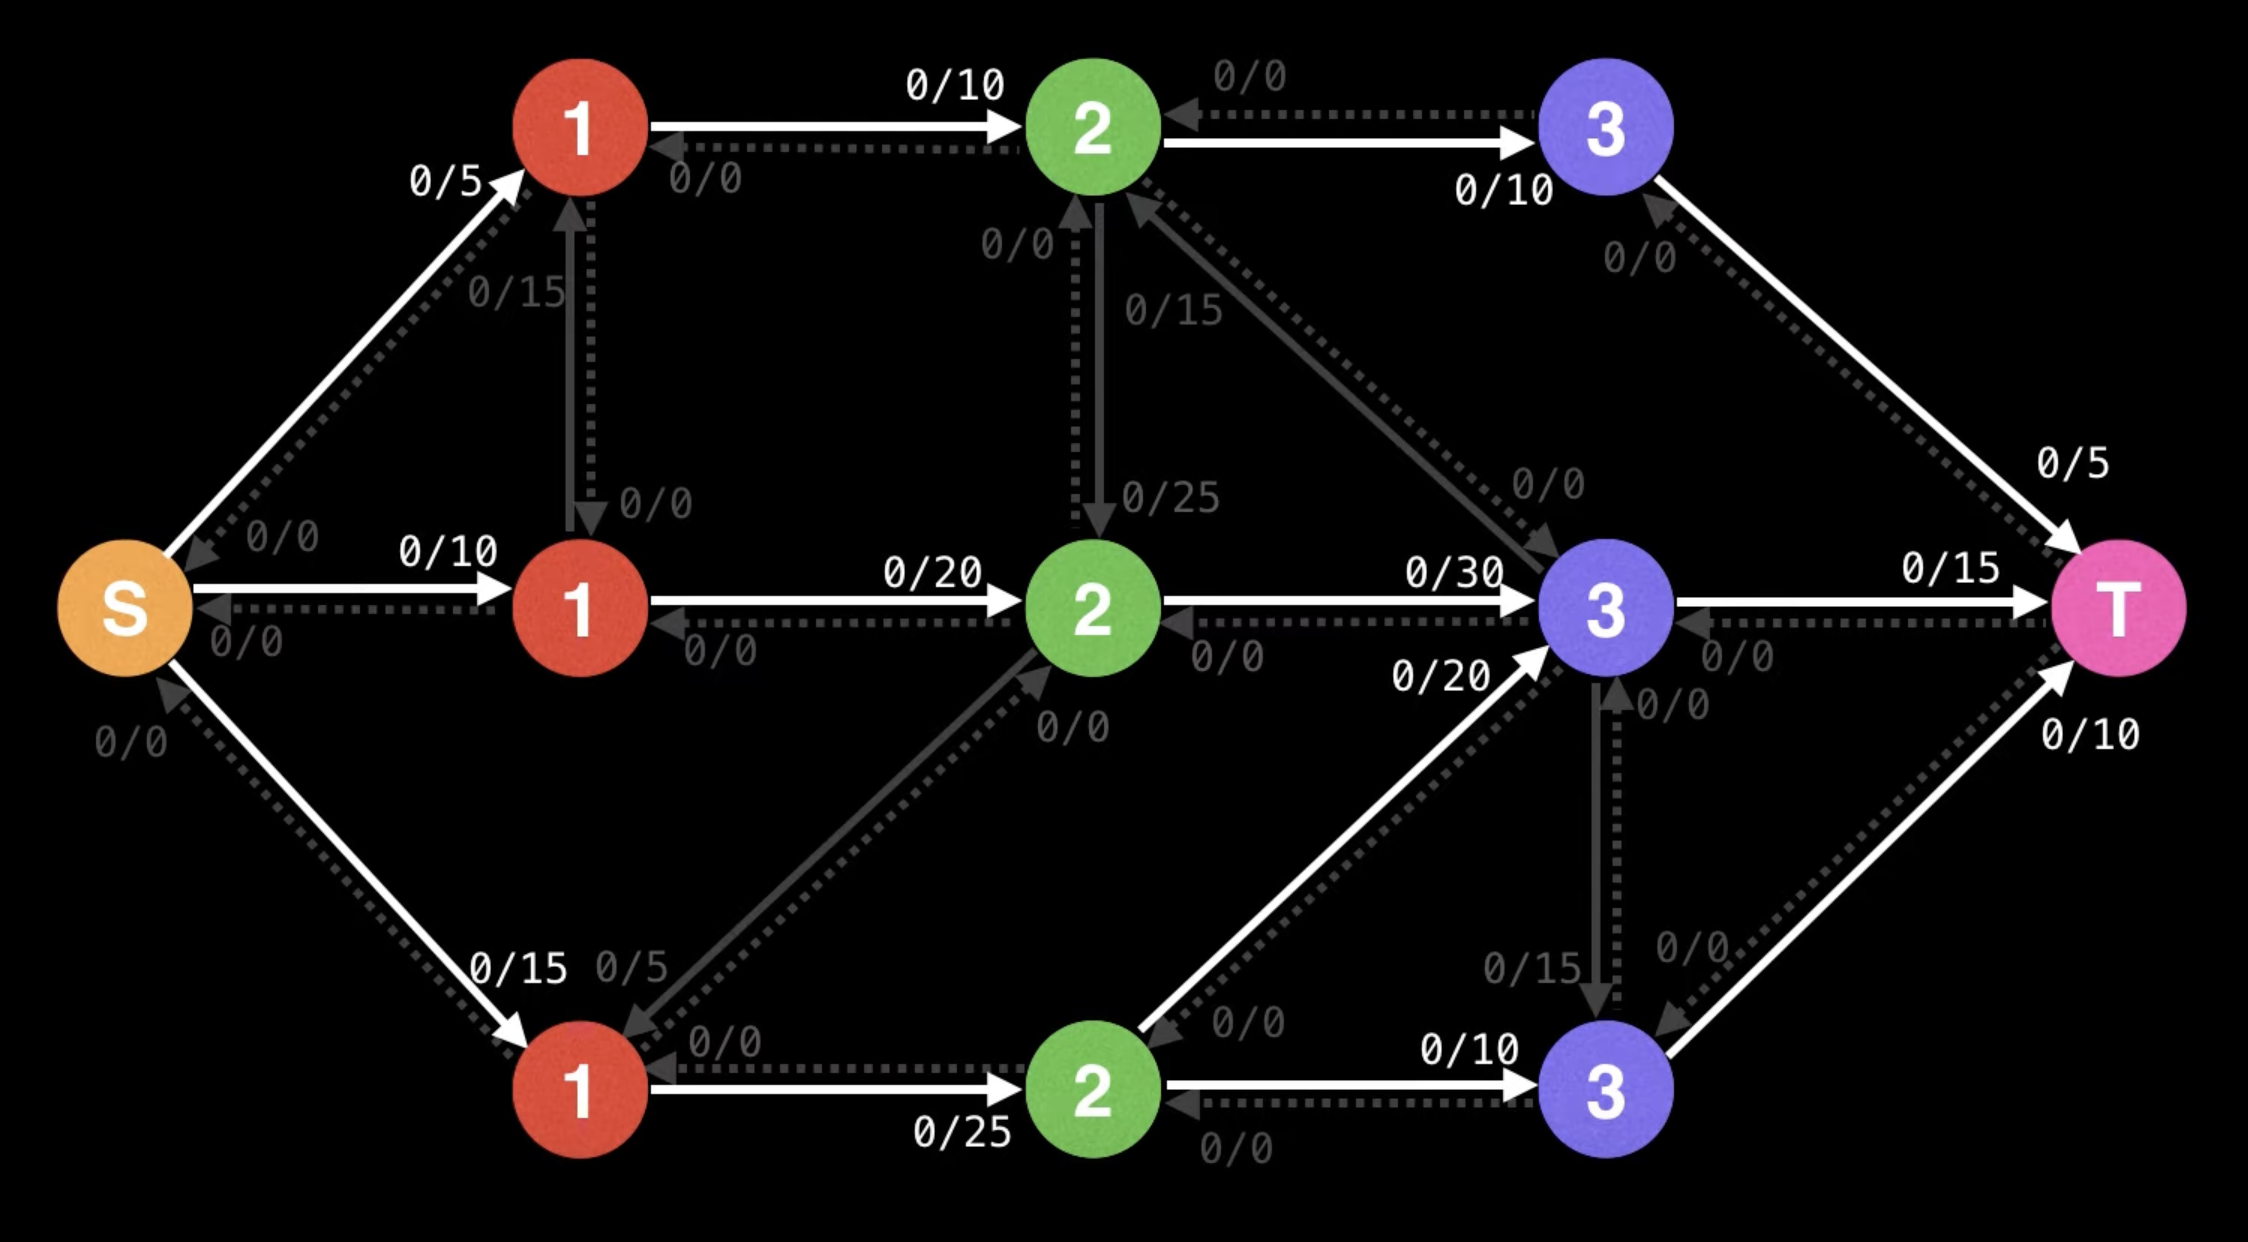
\includegraphics[height=5.25cm]{images/levelGraph.png}\\
    \textit{source: \href{https://www.youtube.com/watch?v=M6cm8UeeziI&t=2s}{Dinic's Algorithm by WilliamFriset}}
\end{center}
In questo modo si riduce il costo dell'algorimo da $O(n^2m)$ per Edmonds Karp a $O(nm^2)$
\paragraph{Altri link utili}\begin{enumerate}
    \item \href{http://courses.csail.mit.edu/6.854/16/Notes/n10-blocking_flows.html}{Lecture from MIT}
    \item \href{https://en.wikipedia.org/wiki/Dinic%27s_algorithm}{Wikipedia}
\end{enumerate}
\newpage

\section{Goldberg-Rao}
\label{gbr}
Ottimizzando il \nameref{dnc}, l'algoritmo di Goldberg-Rao riesce ad ottenere un \textbf{costo computazionale} di $\tilde{O}(\min\{n^{1/2}, m^{2/3}\} \cdot m)$ \\(ovvero $O(\min\{n^{1/2}, m^{2/3}\} \cdot m \cdot \log n \cdot \log nU )$)
su un Network a con capacità intera.
\paragraph*{Dettagli di notazione:}
Nella sezione 2.2 useremo la segue notazione:
\begin{itemize}
    \item $\Lambda = \min\{n^{1/2}, m^{2/3}\}$
\end{itemize}

\subsection{Idea}
    \subparagraph{}
    Alla base dell' ottimizzazione c'è l'idea di \textbf{contrarre} il Network secondo certi specifici parametri.
    L'algoritmo si basa su \nameref{VDL} e introduce una nuova \textbf{length function} \underline{binaria}: $\bar{l}((v,w)): E\rightarrow \{0,1\}$.\\
    La nuova length function assegna valore zero a tutti gli archi che soddisfano certi requisiti di capacità (che descriveremo meglio in seguito).
    \subparagraph{}
    Azzerare la lunghezza degli archi che collegano due o più nodi ci permette di considerarli come un unico nodo. 
    Dunque contraendo le componenti connesse da archi di lunghezza 0 è possibile ridurre in maniera significativa il numero di incrementi di flusso e quindi il costo computazionale dell'algoritmo.

\subsection{Il parametro $\Delta$}
    \subparagraph{}
    Il problema di contrarre il grafo consiste nel fatto che quando immettiamo il flow dalla sorgente al pozzo dobbiamo essere sicuri che tale flow rispetti i vincoli di capacità degli archi originali che ora sono contratti.
    Per assicurarci che i vincoli vengano rispettati si utilizza una certa quantità $\Delta$ che funge da \textit{upper bound} all'incremento di flow e da \textit{lower bound} alla capacità degli archi \textit{zero-length}. 
    \subparagraph{}
    Incrementando il flusso di al massimo $\Delta$ siamo sicuri di rispettare i vincoli di capacità ma non siamo più sicuri che il flusso sia bloccante.
    Dunque dobbiamo scegliere il valore da dare a $\Delta$ in maniera tale che il numero di incrementi sia ragionevolmente piccolo in modo da garantirci il costo computazionale desiderato.

\subsection{Stopping condition}
    L'algoritmo termina quando la differenza tra il flow corrente e quello massimo raggiungibile $F$ diventa minore di 1.
    Dato che le capacità del Network sono tutte intere ciò ci assicura di aver raggiunto il massimo flusso possibile.
    Un primo valore utile per $F$ corrisponde a $F = n\cdot U_{max}$

\subsection{Scheletro dell'algoritmo}
    Possiamo ora descrivere uno scheletro dell'algoritmo come segue:
    \begin{algo}{Goldberg-Rao}{}
        while $F \ge 1$:\begin{enumerate}
            \item Aggiorna il bound $\Delta$, la length function $\bar{l}$, la distance labels $d_{\bar{l}}$;
            \item Contrai i componenti fortemente connessi di archi \textit{zero-length}
            \item Determina l'Admissible graph $A(f, \bar{l},d_{\bar{l}} )$
            \item Trova un flusso in $A(f, \bar{l},d_{\bar{l}} )$ che sia bloccante o di valore $\Delta$
            \item Somma il nuovo flusso trovato con quello ottenuto fin'ora 
            \item Aggiorna il valore di $F$
        \end{enumerate}
        Ritorna il flusso finale 
    \end{algo}
    \textit{NOTA:} Il punto 4 fa riferimento al modo di trovare un flusso bloccante come nel \nameref{dnc}, ciò procedere per incrementi sugli shortest path finché non si raggiunge un flusso bloccante o di valore $\Delta$.
\subsection{Stimare il residual flow}
    Sappiamo già che la capacità residua di ogni taglio $r(S,T)$ rappresenta un \textit{upper bound} al max flow.
    Per stimare il flow residuo molto rapidamente e efficacemente possiamo analizzare i \nameref{cancut}.

    \begin{lemma}{min $r(S_k,T_k)$ in $O(m)$ time}{}
        Il taglio canonico di capacità minima può essere trovato in tempo $O(m)$
    \end{lemma}
    \begin{proof}
        Sfruttiamo il fatto che ogni arco ha lunghezza al massimo $1$, dunque può attraversare al massimo un taglio canonico.
        \begin{itemize}[noitemsep]
            \item Inizializziamo a zero ogni $r(S_k,T_k)$
            \item per ogni $(v,w) \in V$:
            \begin{itemize}
                \item se $d(v) > d(w)$: $r(S_k,T_k) += r(v,w)$
            \end{itemize}
            \item $return\ \min r(S_k,T_k)$
        \end{itemize}
        La correttezza e il costo computazionale di questa routine è piuttosto immediato
    \end{proof}
    Per gestire il costo computazionale bisogna assicurarsi che il valore di $F$ scenda abbastanza in fretta senza appesantire l'algoritmo.\\
    Possiamo raggruppare tutte le iterazioni dell'algoritmo in \textbf{fasi} e aggiornare il valore di $F$ al taglio canonico minimo solo all'inizio di una nuova fase. 
    Ogni fase parte da quando aggiorniamo il valore di $F$ fino a quando\\$\min r(S_k,T_k)\le F/2$.\\
    In questo modo dopo al massimo $\log nU_{max}$ fasi l'algoritmo termina
\subsection{Binary length function}
    Il metodo del blocking flow del Goldberg-Rao riprende da quello di Dinics con importanti modifiche per assicurarsi che: 
    \begin{itemize}[nolistsep]
        \item Il flusso aumenti in maniera significativa ad ogni iterazione 
        \item Dopo ogni raggiungimento di flusso bloccante, la distanza tra $s$ e $t$ aumenti.
    \end{itemize} 
    Allo scopo di raggiungere il costo computazionale desiderato.

    \subparagraph*{} Come già accennato abbiamo bisogno di un upper bound $\Delta$ per rispettare i vincoli di capacità, ma abbiamo anche bisogno che gli incrementi di flussi non bloccanti siano al massimo $\Lambda$ dunque possiamo inizializzare:
    \[\Delta= \lceil F/\Lambda \rceil \]
    La funzione binaria di base è la seguente:
    \[l(u.w) = \left \{ \begin{array}{ll}
        0 & r_{vw} \ge 3\Delta\\
        1 & altrimenti
    \end{array} \right .\]
    dunque archi con larga capacità avranno distanza zero. Tuttavia per raggiungere il costo desiderato è necessario apportare una modifica a tale funzione.
    \begin{definition}{Special Arc}{}
        Un arco $(v,w)$ si dice \textbf{speciale} se soddisfa tutti i seguenti requisiti:
        \begin{itemize}
            \item $2\Delta \le r_{v,w} < 3\Delta$
            \item $d(v) = d(w)$
            \item $r_{wv} \ge 3\Delta$
        \end{itemize}
    \end{definition}    
    La funzione modificata prende in considerazione anche gli archi binari:
    \[\bar{l}(u.w) = \left \{ \begin{array}{ll}
        0 & r_{vw} \ge 3\Delta \lor specialArc((v,w))\\
        1 & altrimenti
    \end{array} \right .\]
\textit{NOTA: Introdurre gli specialArc non modifica la distance labeling: $d_l = d_{\bar{l}}$}

    \begin{lemma}[label = fixCont]{Da contratto a originale}{}
        
        Supponiamo di avere contratto il Network originale come descritto fin'ora, e di aver instradato un flusso $f$ attraverso il grafo contratto.
        \paragraph*{}
        Il costo computazionale di adattare questo flusso attraverso il grafo originale è $O(m)$
    \end{lemma}
    \begin{proof}\begin{enumerate}[nolistsep]
        \item Scegliamo un vertice qualsiasi in ogni componente contratta.
        \item Formiamo un in-tree e un out-tree da con radice nei vertici scelti. 
        \item Dall'in-tree instradiamo il flusso positivo fino alla radice 
        \item Dall'out-tree riconvogliamo il flusso in entrata dalla radice a tutti altri nodi connessi.
    \end{enumerate}
    Dato che il flusso massimo che instradiamo è $\Delta$ e tutti i nodi nei componenti contratti hanno costo almeno $2\Delta$ siamo sicuri che il flusso rispetti le capacità del Network.
    Risulta immediato che tale metodo abbia costo direttamente proporzionale al numero di archi nei componenti connessi.
    \QED
    \end{proof}

    \paragraph*{}Nel Dinic's Algorithm la dimostrazione che il flusso bloccante aumenti strettamente la distanza tra $s$ e $t$ è piuttosto scontata.
    Non si può dire la stessa cosa nel caso del Goldberg-Rao data la presenza di archi di lunghezza zero. Pertanto risulta essenziale la dimostrazione del seguente teorema per assicurarsi che l'algoritmo termini.
    \begin{theo}{Blocking flow with binary length}{}
        Sia $\bar{f}$ un flow in $A(f,\bar{l}, d_l)$, sia $f' = f + \bar{f}$ il flow incrementato e sia 
        $l'$  la length function corrispondente a $f'$. Allora:
        \begin{enumerate}
            \item $d_l$ è una distance lebeling rispetto a $l'$
            \item $d_{l'}(s) \ge d_l(s)$
            \item  se $\bar{f}$ è bloccante $\implies$ $d_{l'}(s) > d_l(s)$
        \end{enumerate}
    \end{theo}
    \begin{proof}
        \textbf{\underline{1. $d_l$ è una distance lebeling rispetto a $l'$}}
            Per definizione di distance labeling $d_l(v) \le d_l(w) + \bar{l}(v,w)$ (ricordando che $d_l = d_{\bar{l}}$) 
            dobbiamo quindi dimostrare che  $d_l(v) \le d_l(w) + l'(v,w)$.\\
            Questo ciò è banalmente vero se $d_l(v) \le d_l(w)$.\\
            Se $d_l(v) > d_l(w)$ ovvero $d_{\bar{l}}(v) > d_{\bar{l}}(w)$ allora $(w,v)$ non è ammissibile rispetto a $\bar{l}$.\\
            Ciò ci assicura che $u_{f'}(v,w)\le u_{f}(v,w)$ il che implica che \colorbox{yellow!40!white}{$l'(v,w)\ge \bar{l}(v,w)$} da cui segue lo statement.

            \paragraph*{\underline{2. $d_{l'}(s) \ge d_l(s)$}}

            Dimostriamo che il se $L:= {l_0, l_1, ..., l_n}$ l'insieme ordinato di tutte le funzioni di lunghezza
            calcolate tra le iterazioni dell'algoritmo allora per qualsiasi $0 \le i \le j \le n \implies d_{l_i}(s) \le d_{l_j}(s)$.\\
            Distinguiamo le due iterazioni come:
            \begin{itemize}
                \item Nell'iterazione $i$\\
                Sia $l(u,v) = l_i(u,v)$ la funzione di lunghezza e $d(x) = d_{l_i}(x)$ quella di distanza, insieme al flusso definiscono $A(f, l_i, d_{l_i})$.\\ Sia $\Gamma$ l'$s\rightarrow t$ shortest path in $A: \Gamma \subseteq A$
                \item Nell'iterazione $j$\\
                Sia $l'(u,v) = l_j(u,v)$ la funzione di lunghezza e $d'(x) = d_{l_j}(x)$ quella di distanza, insieme al flusso definiscono $A'(f, l_j, d_{l_j})$.\\ Sia $\Gamma'$ l'$s\rightarrow t$ shortest path in $A': \Gamma' \subseteq A'$
            \end{itemize}
            
            Supponiamo per assurdo che esistano due iterazioni $0 \le i\le j :$\\$ d(s) > d'(s)$:
            \[\implies \exists \Gamma s\rightarrow t,\ \Gamma ' \ s \rightarrow t : \sum_{(v,w)\in \Gamma} l(v,w) \ge \sum_{(v,w)\in \Gamma'} l'(v,w)\]
            Ovvero andando avanti con le iterazioni $s$ e $t$ si sono avvicinati.\\
            Escludiamo subito il caso in cui $\Gamma = \Gamma'$ in quanto
            \[\forall (v,w)\in A\cap A',\  l(v,w) \le l'(v,w)\implies l(\Gamma)\ \le\ l'(\Gamma')\]
            \begin{center}
                \textit{NOTA: $l(\Gamma) = \sum_{(v,w)\in \Gamma} l(v,w)$}
            \end{center}
            Consideriamo ora $\Gamma$ e $\Gamma'$. Sia $w$ l'ultimo nodo in $\Gamma$ per cui è vero che $d(w)> d'(w)$ e sia $x$ il nodo che lo segue:
            \[w \in \Gamma : d(w) > d'(w) \land \exists x = succ_\Gamma(w) : d(x)\le d'(x)\]
            $w$ e $x$ sono sempre ben definiti perché $d(s)>d'(s)$ per ipotesi e $d(t) = d'(t) = 0$ per definizione.
            Dunque esiste in $\Gamma'$ un arco $(w,y)$ con $y \not = x$ tale che $d'(y) < d'(x)$. $x \not = y$ perché se fossero lo stesso nodo allora \[d'(w) = d'(x) + l'(w,x)\ge d(w)\]
                che contraddice le ipotesi\\
            Ricomponendo il tutto, sappiamo che:
            \begin{enumerate}
                \item $d(w)>d'(w) \iff d(x) + l(w,x) > d'(y) + l'(w,y)$ \\Non conosciamo la distanza $d(y)$ ma sappiamo che:
                \[d'(y) = \sum_{(a,b)\in y-t\subseteq \Gamma'}l'(a,b) \ge \sum_{(a,b)\in y-t\subseteq \Gamma'}l(a,b) \]
                Quindi il percorso all'iterazione $j$ è maggiore o uguale a quello dell'iterazione $i$.
                \item $d(y) +l(w,y) \le d'(y) +l'(w,y) < d(x) +l(w,x)$  
            \end{enumerate}
            Ma noi sappiamo che $d(w) = d(x) +l(w,x)$ il che è \textbf{assurdo} perché non è la distanza minima di $w\rightarrow t$ in quanto è maggiore di 
            $d(y) +l(w,y)$. 
            
            Sappiamo per certo che il percorso $w-y\rightarrow t$ esiste in $A$ proprio perché (a meno che non ne esista uno più corto) rappresenta il percorso con distanza minima da $w\rightarrow t$.

            Dall'assurdo, le uniche conclusioni sono che o il percorso che passa per $y$ non era raggiungibile all'iterazione $i$ e quindi è impossibile raggiungerlo successivamente, 
            oppure se esiste un percorso $s\rightarrow t$ all'iterazione $j$ minore di quello all'iterazione $i$, abbiamo sbagliato a considerare quello all'iterazione $i$.

        
            \paragraph*{\underline{3. Se $\bar{f}$ è bloccante allora $d_l(s) < d_{l'}(s)$}}

            Per mostrare che il flow bloccante aumenta la distanza del nodo $s$ definiamo il la seguente dicitura:
            \[c(v,w):= d_l(w)-d_l(v) + l'(v,w)\]
            che rappresenta il cambiamento di lunghezza di un arco che collega due nodi adiacenti.
            Possiamo affermare che:
            \[\forall (v,w)\in E,\ c(v,w)\ge 0\]
            dato che $l'(v,w)\ge l(v,w)\implies$
            \[ d_l(w)-d_l(v) < 0 \iff l(v,w) = 1 \implies l'(v,w) = 1\]
            Consideriamo ora un qualsiasi percorso $\Gamma$ in $G_{f'}$, la lunghezza del percorso è uguale a: 
            \[l'(\Gamma) = d_l(s)+c(\Gamma)\]
            Per mostrare quindi che il percorso è più lungo basta mostrare che 
            \[\forall shortest\ s-t\ path\ \Gamma \in G_{f'}\implies \exists (v,w)\in \Gamma | c(v,w) > 0\]
            Abbiamo ora uno strumento per mostrare che il flusso bloccante aumenta la distanza di $s$.

            \begin{example}{}{}

            \begin{tabular}{c|c}
                \multicolumn{2}{c}{Un semplice esempio grafico per visualizzare meglio quanto dichiarato}\\
                \\
                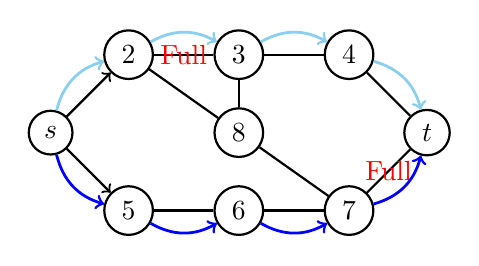
\begin{tikzpicture}[node distance={14mm}, thick , main/.style = {draw, circle}] 
                \node[main] (1) at (0,0) {$s$}; 
                \node[main] (2) [above right of=1] {$2$};
                \node[main] (3) [right of=2] {$3$};
                \node[main] (4) [right of=3] {$4$};
                \node[main] (5) [below right of=1] {$5$};
                \node[main] (6) [right of=5] {$6$};
                \node[main] (7) [right of=6] {$7$};
                \node[main] (9) [below right of=4] {$t$};
                \node[main] (8) at ($(1)!0.5!(9)$) {$8$};
                %Admissible
                \draw[->] (1) to (2);
                \draw[-] (2) to [red, midway] node {Full} (3);
                \draw[-] (3) to (4);
                \draw[-] (4) to (9);
                \draw[-] (3) to (8);
                \draw[-] (2) to (8);
                \draw[-] (8) to (7);
                \draw[->] (1) to (5);
                \draw[-] (5) to (6);
                \draw[-] (6) to (7);
                \draw[-] (7) to [red, midway] node {Full} (9);
                
                %paths
                \draw[->,line width=1 pt] (1)[babyblue, bend left] to (2);
                \draw[->,line width=1 pt] (2)[babyblue, bend left] to (3);
                \draw[->,line width=1 pt] (3)[babyblue, bend left] to (4);
                \draw[->,line width=1 pt] (4)[babyblue, bend left] to (9);
            
                \draw[->,line width=1 pt] (1)[blue, bend right] to (5);
                \draw[->,line width=1 pt] (5)[blue, bend right] to (6);
                \draw[->,line width=1 pt] (6)[blue, bend right] to (7);
                \draw[->,line width=1 pt] (7)[blue, bend right] to (9);

            
            \end{tikzpicture} 
            &
            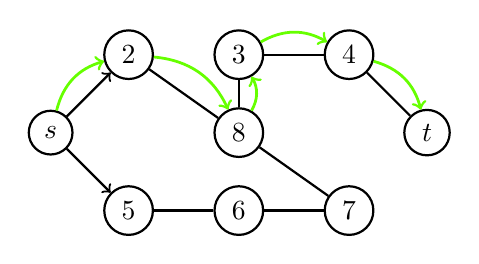
\begin{tikzpicture}[node distance={14mm}, thick , main/.style = {draw, circle}] 
                \node[main] (1) at (0,0) {$s$}; 
                \node[main] (2) [above right of=1] {$2$};
                \node[main] (3) [right of=2] {$3$};
                \node[main] (4) [right of=3] {$4$};
                \node[main] (5) [below right of=1] {$5$};
                \node[main] (6) [right of=5] {$6$};
                \node[main] (7) [right of=6] {$7$};
                \node[main] (9) [below right of=4] {$t$};
                \node[main] (8) at ($(1)!0.5!(9)$) {$8$};
                %Admissible
                \draw[->] (1) to (2);
                \draw[-] (3) to (4);
                \draw[-] (4) to (9);
                \draw[-] (3) to (8);
                \draw[-] (2) to (8);
                \draw[-] (8) to (7);
                \draw[->] (1) to (5);
                \draw[-] (5) to (6);
                \draw[-] (6) to (7);
                
                \draw[->,line width=1 pt] (1)[brightgreen, bend left] to (2);
                \draw[->,line width=1 pt] (2)[brightgreen, bend left] to (8);
                \draw[->,line width=1 pt] (8)[brightgreen, bend right] to (3);
                \draw[->,line width=1 pt] (3)[brightgreen, bend left] to (4);
                \draw[->,line width=1 pt] (4)[brightgreen, bend left] to (9);

            \end{tikzpicture}\\
            In \textbf{\color{babyblue}{azzurro}} $f$ e in  & In \textbf{\color{brightgreen}{verde}} lo \textit{shortest path} $\Gamma$ in $G_{f'}$\\
            \textbf{\color{blue}{blu}} $\bar{f}$ in $A(f,\bar{l}, d_l)$ &
\end{tabular}
\end{example}
    Dato che $\bar{f}$ è bloccate in $A(f,\bar{l}, d_l)$, $\Gamma$ deve contenere un arco $(v,w)$ non presente in in $A(f,\bar{l}, d_l)$.
    
    Possiamo in oltre affermare che $d_l(v)\le d_l(w)$ o perché $(v,w) \in G_f$ ma allora se $d_l(v)> d_l(w)$ avremmo $(v,w) \in A(f,\bar{l}, d_l)$
    oppure perché $(v,w) \not \in G_f$ ma appare in $G_{f'}$ e ciò è possibile solo se incremento il flusso nella direzione opposta per far apparire l'arco residuo. Dunque $(w,v) \in A(f,\bar{l}, d_l)$ il che implica che $d_l(v)\le d_l(w)$.

    Supponiamo ora per assurdo che $c(v,w) = 0$, dunque $d_l(v) = d_l(w)$ e $l'(v,w) = 0$.
    Il fatto che $(v,w)$ non sia in $A(f,\bar{l}, d_l)$ implica che o $(v,w)$ non sia in $G_f$, ma allora abbiamo mostrato già che l'arco opposto $(w,v)\in A(f,\bar{l}, d_l)$, 
    oppure che $(v,w) \in G_f$ e non rispetta i requisiti di distance labeling per appartenere all'\nameref{AdmissibleGraph} $A(f,\bar{l}, d_l)$.\\
    Dato che $d_l(v) = d_l(w)$ allora $l(v,w) = 1$. Si nota $1 = l(v,w) > l'(v,w) = 0$ implica che ho incrementato il flusso sull'arco opposto $(w,v)$.\\
    Dunque in ogni caso l'arco $(w,v)\in A(f,\bar{l}, d_l)$.

    Come già mostrato in precedenza, dato che $d_l(v) = d_l(w)$, \[(w,v)\in A(f,\bar{l}, d_l) \iff l(w,v) = 0\]
    Concludiamo quindi che: 
    \begin{itemize}
        \item Durante gli incrementi di flusso abbiamo immesso un flow (di valore al massimo $\Delta$) attraverso l'arco $(w,v)$
        \item $u_f(w,v) \ge 3\Delta$ perché $l(w,v) = 0$
        \item Dopo questo incremento abbiamo: $r_{f'}(v,w) \ge 0$ perché  $l'(v,w) = 0$
        \item Quindi $u_f(v,w) \ge 2\Delta$
        \item Ma allora l'arco $(v,w)$ era un \textit{arco speciale} già prima dell'incremento, in quanto $d_l(v) = d_l(w) \land u_f(w,v) \ge 3\Delta \land u_f(v,w) \ge 2\Delta$
    \end{itemize}
    Concludiamo quindi che: 
    \[d_l(v) = d_l(w) \implies d_{\bar{l}}(v) = d_{\bar{l}}(w) \land \bar{l}(v,w) = 0 \implies (v,w) \in A(f,\bar{l}, d_l)\]
    Il che è assurdo 
    \QED
    \end{proof}
    \subsection{Costo computazionale}
    Dimostrata la correttezza del codice, segue il costo computazionale:
    \subsubsection{Costo di una fase}
    Prima di addentrarci nel costo di una fase, rivediamo la struttura dell'algoritmo descritto fino ad ora.
    \begin{verbatim}
    def Goldberg_Rao_Algorithm(Network network)
        F = U*n
        Delta = F/Lambda
        f = 0
        while F >= 1:
            l = update_length(n, Delta)
            d_l = distanceLabel(network, l)
            Gc = collapse(network)
            Ag = admissible_graph(g)
            f' = find_blocking_or_Delta_flow(Ag)
            f = f + f'
            network.fitFlow(f)
            if min_canonical_cut(network).residual() <= F/2: 
                F = min_canonical_cut(network).residual()
                Delta = F/Lambda

        return f
        
    \end{verbatim}
    \begin{remark}
        {Costo da raggiungere}{}
        Il costo dichiarato in partenza è in:
        \[O(\min \{m^{2/3},\ n^{1/2}\}\cdot m \log n\log m U_{max})\]
        utilizzando strutture dati più avanzate, si può raggiungere il costo di:
        \[O(\min \{m^{2/3},\ n^{1/2}\}\cdot m \log \frac{n^2}{m}\log U_{max})\]

    \end{remark}
    Abbiamo già notato che il numero di \textbf{fasi} (ovvero il numero di decrementi) di F è nell'ordine di $\log(F)$ ovvero $log(m U_{max})$.
    Il costo per calcolare il min canonical cut e per adattare il flow al network sono entrambi in $O(m)$.
    Resta però da analizzare il costo di ogni fase, cioè quanto in fretta il min canonical cut si dimezza.
    \begin{lemma}
        {}{}
        La capacità minima di un canonical cut $(\bar{S}, \bar{T})$ soddisfa
        \[u_f(\bar{S}, \bar{T})\le \frac{mM}{d_l(s)}\]
        dove M rappresenta l'arco di lunghezza uno con più capacità
    \end{lemma}
    \begin{proof}
        Risulta evidente che il il modo migliore in cui si può massimizzare la capacita del taglio canonico minimo è supponendo che tutti gli archi abbiano la capacità dell'arco di capacità maggiore e poi dividere equamente gli archi tra i vari tagli.
    \QED
    \end{proof}

    Da questa prima stima segue il corollario
    \begin{corollary}{}{}
    Durante ogni fase ci sono al massimo $O(\Lambda)$ blocking flow incrementi.
    \end{corollary}
    \begin{proof}
        Supponiamo che $\Lambda = m^{1/2}$ dato che abbiamo dimostrato che ogni blocking flow incrementa $d(s)$ di almeno uno, siamo sicuri che dopo $6\lceil \Lambda\rceil$ incrementi $d_l(s) \ge 6 m^{1/2}$.
        Dunque possiamo prendere la stima nel lemma e affermare che:
        \[ u_f(\bar{S}, \bar{T})\le \frac{mM}{d_l(s)}\le \frac{3m}{d_l(s)}\Delta\le \frac{3m}{6m^{1/2}}\frac{F}{m^{1/2}} = \frac{F}{2}\]
        Dunque dopo $\lceil \Lambda\rceil$ la fase termina.\\
        Per $\Lambda = n^{2/3}$ la dimostrazione è analoga e porta alla stessa conclusione. 
        In conclusione, il costo di ogni fase è in ordine di $O(\Lambda)$ \QED
    \end{proof}
    
    L'ultimo collo di bottiglia è rappresentato dal costo di trovare un blocking flow o di valore massimo $\Delta$ (computazionalmente equivalenti):
    il che richiederebbe un costo di:
    \begin{itemize}
        \item $O(mn)$ in un approccio naive;
        \item $O(m\log n)$ utilizzando i dynamic trees;
        \item $O(m \log(n^2/m))$ utilizzando i size-bounded dynamic trees;
    \end{itemize}
    Unendo il costo di:
    \begin{itemize}[label=$\times$]
        \item trovare un Blocking flow
        \item le iterazioni in ogni fase
        \item il numero di fasi
        \item gli ulteriori costi in $O(m)$
    \end{itemize}
    Si ottiene il tempo dichiarato.











    \chapter{Prim Algorithm}
Fino ad ora gli algoritmi hanno minimizzato il costo computazionale fino ad arrivare ad un costo $O(nm)$ solo quando il valore di $m$ o $n$ assumeva determinate proporzioni.
Il seguente algoritmo attinge dall'algoritmo \textbf{Goldberg and Rao} modificandone dei passaggi e preservando alcuni concetti per dimostrare però che si può risolvere il problema del max flows in $O(nm)$ per qualunque valore di $n$ e $m$.
\section{Idea}
Il problema viene risolto attraverso una serie di incrementi di flusso come nel Goldberg and Rao ma si rimpiazza il Network residuo del $\Delta$-incremento con una versione più compatta.
l'algoritmo presenta due bottleneck: \begin{enumerate}
    \item creazione della rappresentazione compattata
    \item passaggio dal flow compattato al flow esteso.
\end{enumerate}
\section{Passaggi}

Di seguito la lista dei passaggi che il programma svolge per risolvere il problema in $O(mn)$:
\begin{enumerate}
    \item scegliere un cut $(S,T)$
    \item calcolo del residual graph
    \item calcolo del \textit{abundant graph} (+ chiusura transitiva)
    \item riduzione del residual graph a \textit{strongly compact}
    \item riduzione dello \textit{strongly compact} a \textit{$\Delta$-compact}
\end{enumerate}

La particolarità di questo algoritmo sta nella scelta della modalità di incremento del flusso.
\newpage
\section{Fase di incremento}
Il max-flow flow problem viene risolto attraverso una serie di \textit{fasi di incremento}, vediamo quindi quali sono gli input e gli output di ogni fase:
\begin{itemize}[itemsep=0.5ex]
    \item \textbf{input}
    \begin{enumerate}
        \item un \textit{Flow} $f$
        \item un \textit{Residual Graph} $G_f$, rappresentabile anche come $r: E \rightarrow \mathbb{R}$ la funzione che associa a ogni arco la sua capacità residua
        \item un s-t cut $(S,T)$
    \end{enumerate}
    Possiamo rappresentare l'input con la tripla $(r,S,T)$
    \item \textbf{output}
    \begin{enumerate}
        \item un \textit{Flow} $f'$
        \item un \textit{Residual Graph} $G_f'$
        \item un s-t cut $(S',T')$ tale che $r'(S',T') \le \frac{r(S,T)}{4m}$
    \end{enumerate}
\end{itemize}
Questa fase prende il nome di $\Delta\text{-}improvment\ phase$ dove $\Delta = r(S,T)$.

Questo tipo di incremento viene eseguito, a seconda delle condizioni, o sul network $G$ oppure sul \textit{compact network} $G^c$

\section{$\Delta$-abundant e grafo di abbondanza}
In questa sezione viene presentato il concetto di \textbf{Abbondanza} che in un certo senso sostituisce quello di \textbf{lunghezza} di Goldberg-Rao, che infatti non è sfruttato per la soluzione di Prim.
\begin{definition}{$\Delta$-abundant arc}{}
    Sia $\Delta = r(S,T)$ un arco $(i,j)$ si dice $\Delta$-abbondante se $r_{ij} \ge 2\Delta$ 
     
\end{definition}
\begin{lemma}{}{}
    \label{ab4ever}
    Sia $(r,S,T)$ l'input di una $\Delta\text{-}improvment\ phase$. Se l'arco $(i,j)$ è abbondate prima dell'incremento allora rimmarrà abbondante per tutti gli incrementi successivi.
\end{lemma}
\begin{proof}
    Dato che 
    $\Delta' \le \frac{\Delta}{4m} $ e ricordando che $r_{ij} \ge 2\Delta $ si deduce che 
    allora \[r'_{ij} \ge r_{ij}-\Delta \ge\Delta\ge  2\Delta'\]\QED
\end{proof}

\begin{definition}{Grafo di Abbondanza}{}
    Dato un network $G$ si definisce il suo \textbf{grafo di abbastanza} $G^{ab}$ come: 
    \[G^{ab} := (N(G), \{(i,j)| (i,j)\in E(G)\land r_{ij}\ge 2\Delta\})\]
\end{definition}
\begin{obs}{}{}
    Per il \hyperref[ab4ever]{lemma 7} proseguendo con le iterazioni il grafo di abbondanza può solo acquisire nuovi archi, mai perderli.
\end{obs}

IL grafo di abbondanza è utile in vari modi: 
\begin{enumerate}
    \item Tutti i cicli formati da archi abbondanti vengono \textit{contratti} in un solo nodo
    \item Tutti i nodi che adiacenti solo ad archi abbondanti o di capacità troppo piccola, vengono \textit{compattati}
\end{enumerate}
L'algoritmo mantiene in oltre la chiusura transitiva di tutti i nodi collegati tra loro da un \textbf{abundant path}, ovvero un cammino composto solo da archi abbondanti. \\
Se esiste un abundant path tra il nodi $i$ e $j$, ciò si indica con $i\implies j$, e l'informazione viene mantenuta in una matrice \textbf{M}$_{n\times n}$, dove nella posizione 
\textbf{M}$_{i,j}$ si trova il nodo che precede $j$ nel percorso che parte da $i$. Se durante le iterazioni si creano più percorsi viene comunque mantenuto il primo trovato.

La chiusura transitiva può essere mantenuta in tempo $O(nm)$ utilizzando l'algoritmo di Italiano. 
In questo modo è sempre possibile (vedremo di seguito che contrarre il grafo non lo impedisce e non ne altera il costo) ricostruire un percorso abbondante $P$ in $O(|P|)$
\newpage
\section{Contractions of abundant graph}
Vediamo ora come sfruttare l'abundant graph per contrarre il grafo su cui calcolare il max-flow e rendere l'algoritmo più efficiente.

Analizziamo tre contrazioni di esempio differenti:\\
\\
Supponiamo che esistano due nodi $i$ e $j$ tali che $r_{ij} \ge 2\Delta$ e $r_{ji} \ge 2\Delta$

Possiamo quindi contrarre i due nodi in uno unico che preservi gli archi di entrambi
\[\begin{tabular}{ccc}
    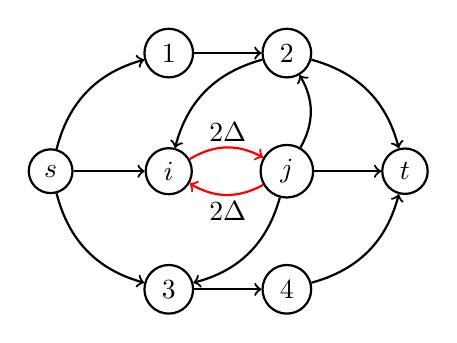
\begin{tikzpicture}[node distance={15mm}, thick , main/.style = {draw, circle}] 
    % Disegna i nodi del grafo
    

    \node[main] (0) {$s$};
    \node[main] (3) [right of= 0 ] {$i$};
    \node[main] (4) [right of=3] {$j$};
    \node[main] (1) [below of = 3 ] {3};
    \node[main] (2) [above of = 3] {$1$};
    
    \node[main] (6) [above of=4] {$2$};
    \node[main] (5) [below of=4] {$4$};
    \node[main] (7) [right of=4] {$t$};
    % Disegna gli archi orientati
    \draw[->] (0) [bend right] to (1);
    \draw[->] (0) [bend left] to (2);
    \draw[->] (0) to (3);
    \draw[->] (3) [red, bend left] to (4);
    \node at (2.25,0.5) {$2\Delta$};
    \node at (2.25,-0.5) {$2\Delta$};
    \draw[->] (4) [red, bend left] to (3);
    
    \draw[->] (2) to (6);
    \draw[->] (4)[bend left] to (1);
    \draw[->] (4)[bend right] to (6);
    \draw[->] (6)[bend right] to (3);
    \draw[->] (4) to (7);
    \draw[->] (1) to (5);
    \draw[->] (6)[bend left] to (7);
    \draw[->] (5)[bend right] to (7);


\end{tikzpicture}&\begin{tikzpicture}
    \node {$\implies$};% Freccia verso destra
    \node at (0,1.4) {};
    \node at (0,-1.6) {};
\end{tikzpicture}  &
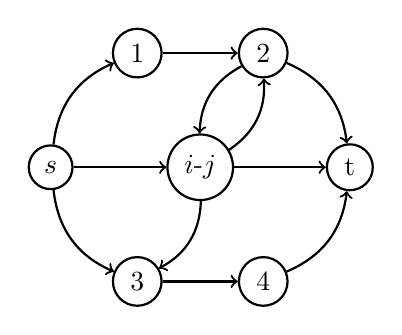
\begin{tikzpicture}[node distance={19mm}, thick , main/.style = {draw, circle}] 
    % Disegna i nodi del grafo
    
    
    \node[main] (m)  {$i$-$j$};
    \node[main] (0) [left of = m ]{$s$};
    \node[main] (1) at (-0.8,1.45) {1};
    
    \node[main] (2) at (0.8,1.45) {$2$};

    \node[main] (3) at (-0.8,-1.45) {$3$};
    \node[main] (4) at (0.8,-1.45) {$4$};

    \node[main] (5) [right of = m] {t};
    % Disegna gli archi orientati

    
    \draw[->] (0) to (m);
    \draw[->] (0)[bend left] to (1);
    \draw[->] (0)[bend right] to (3);

    \draw[->] (1) to (2);

    \draw[->] (2)[bend right] to (m);
    \draw[->] (m)[bend right] to (2);
    \draw[->] (m)[bend left] to (3);
    \draw[->] (2)[bend left] to (5);
    \draw[->] (m) to (5);
    \draw[->] (3) to (4);  
    \draw[->] (4)[bend right] to (5);

\end{tikzpicture}
\end{tabular}\]

È possibile contrarre archi esterni  

\[\begin{tabular}{ccc}
    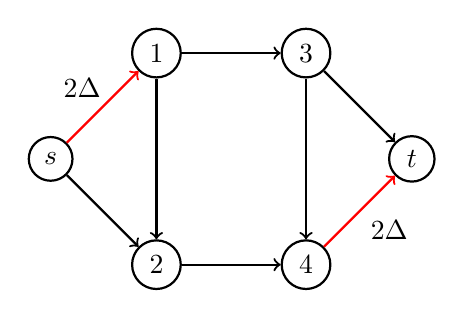
\begin{tikzpicture}[node distance={19mm}, thick , main/.style = {draw, circle}] 
    % Disegna i nodi del grafo
    
    \node[main] (0) {$s$};
    \node[main] (1) [above right of = 0] {1};
    \node[main] (2) [below right of = 0] {2};
    \node[main] (3) [right of = 1] {3};
    \node[main] (4) [right of = 2] {4};
    \node[main] (5) [below right of = 3] {$t$};
    
    \draw[->] (0) [red] to (1);
    \draw[->] (1) to (3);
    \draw[->] (0) to (2);
    \draw[->] (2) to (4);
    \draw[->] (3) to (5);
    \draw[->] (4) [red] to (5);
    \draw[->] (1) to (2);
    \draw[->] (3) to (4);

    \node at (0.4,0.9) {$2\Delta$};
    \node at (4.3,-0.9) {$2\Delta$};

\end{tikzpicture}&\begin{tikzpicture}
    \node {$\implies$};% Freccia verso destra
    \node at (0,1.4) {};
    \node at (0,-1.6) {};
\end{tikzpicture}  &
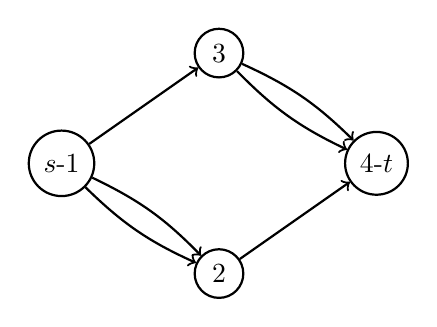
\begin{tikzpicture}[node distance={19mm}, thick , main/.style = {draw, circle}] 
    % Disegna i nodi del grafo
    \node[main] (0) {$s$-$1$};
    \node[main] (3) at (2,1.4) {$3$};
    \node[main] (2) at (2,-1.4) {$2$};
    \node[main] (4) at (4,0) {4-$t$};

    \draw[->] (0) to (3);
    \draw[->] (0) [bend left = 10] to (2);
    \draw[->] (0) [bend right = 10] to (2);
    
    
    \draw[->] (2) to (4);
    \draw[->] (3) [bend left = 10] to (4);
    \draw[->] (3) [bend right = 10] to (4);
    

\end{tikzpicture}
\end{tabular}\]

E dunque tutti i cicli abbondanti

\[\begin{tabular}{ccc}
    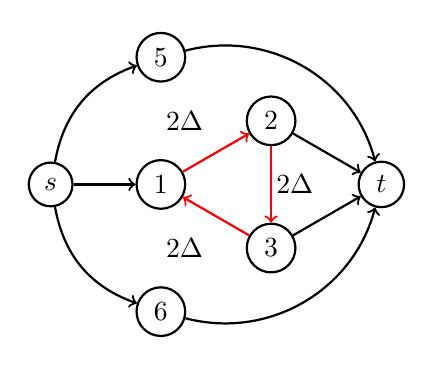
\begin{tikzpicture}[node distance={18mm}, thick , main/.style = {draw, circle}] 
    % Disegna i nodi del grafo
    
    \node[main] (0) {$s$};
    \node[main] (1) at (1*1.4,0) {1};
    \node[main] (2) at (2*1.4,0.577*1.4) {2};
    \node[main] (3) at (2*1.4,-0.577*1.4) {3};
    \node[main] (4) at (3*1.4,0) {$t$};
    \node[main] (5) at (1*1.4,1.154*1.4) {$5$};
    \node[main] (6) at (1*1.4,-1.154*1.4) {$6$};

    \draw[->] (0) [bend left] to (5);
    \draw[->] (0) [bend right] to (6);
    \draw[->] (0)  to (1);
    \draw[->] (1)[red]  to (2);
    \draw[->] (2)[red]  to (3);
    \draw[->] (3)[red]  to (1);
    \draw[->] (2)  to (4);
    \draw[->] (3)  to (4);
    \draw[->] (5) [bend left = 45] to (4);
    \draw[->] (6) [bend right = 45] to (4);

    \node at (3.1,0) {$2\Delta$};
    \node at (1.7,0.577*1.4) {$2\Delta$};
    \node at (1.7,-0.577*1.4) {$2\Delta$};
    

\end{tikzpicture}&\begin{tikzpicture}
    \node {$\implies$};% Freccia verso destra
    \node at (0,1.4) {};
    \node at (0,-1.6) {};
\end{tikzpicture}  &
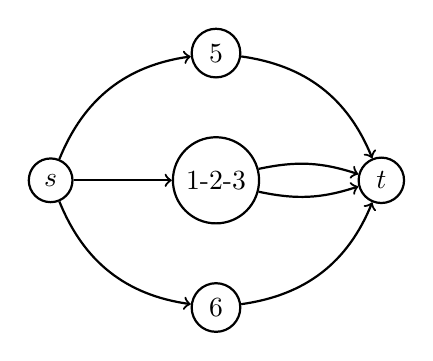
\begin{tikzpicture}[node distance={19mm}, thick , main/.style = {draw, circle}] 
    % Disegna i nodi del grafo
    \node[main] (0) {$s$};
    \node[main] (1) at (1.5*1.4,0) {1-2-3};
    \node[main] (5) at (1.5*1.4,1.154*1.4) {$5$};
    \node[main] (6) at (1.5*1.4,-1.154*1.4) {$6$};
    \node[main] (4) at (3*1.4,0) {$t$};

    \draw[->] (0) [bend left] to (5);
    \draw[->] (5) [bend left] to (4);
    \draw[->] (0) [bend right] to (6);
    \draw[->] (6) [bend right] to (4);

    \draw[->] (0) to (1);
    \draw[->] (1) [bend left= 15] to (4);
    \draw[->] (1) [bend right = 15] to (4);

\end{tikzpicture}
\end{tabular}\]
\begin{obs}{Violazioni della conservazione del flusso}{}
    È possibile che quando il grafo contratto verrà riespanso venga violata la legge di conservazione del flusso. 
    
    Tuttavia si tratta di una violazione minore di $2\Delta$ unità dunque, come mostrato da \hyperref[fixCont]{Goldberg e Rao} la contrazione, l'espansione e l'adattamento per la conservazione del flusso possono essere eseguiti in tempo $O(m)$. 
\end{obs}
\section{The compact network}
Oltre alla contrazione del grafo è necessario eseguire un'altra trasformazione, la \textit{compattazione}.
Per ottenere un grafo compatto mostriamo prima come ottenere una versione intermedia ovvero lo \textbf{strongly compact network}.

\noindentÈ importante comprendere la differenza tra contrarre e compattare:

Se nella contrazione viene creato un nodo unico che rappresenta il ciclo abbondate e vengono preservati gli archi originali non appartenenti al ciclo, 
quando si compatta un grafo viene \underline{eliminato} un nodo che ha tutti gli archi adiacenti abbondanti e gli archi eliminanti di conseguenza vengono sostituiti da pseudo archi.

\[\begin{tabular}{ccc}
    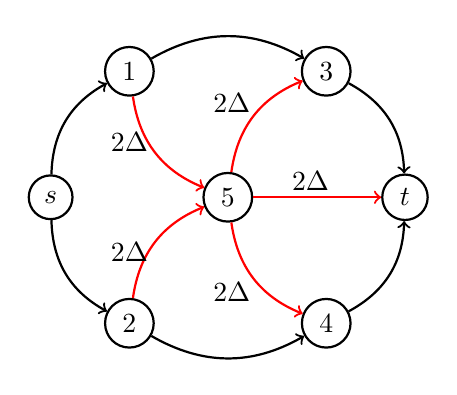
\begin{tikzpicture}[node distance={18mm}, thick , main/.style = {draw, circle}] 
    % Disegna i nodi del grafo
    
    \node[main] (0) {$s$};
    \node[main] (1) at (1, 1.6) {1};
    \node[main] (2) at (1, -1.6) {2};
    \node[main] (3) at (3.5, 1.6) {3};
    \node[main] (4) at (3.5, -1.6) {4};
    \node[main] (6) at (2.25,0) {5};
    \node[main] (5) at (4.5, 0) {$t$};

    \draw[->] (0)[bend left] to (1);
    \draw[->] (0)[bend right] to (2);
    \draw[->] (1)[bend left] to (3);
    \draw[->] (2)[bend right] to (4);
    \draw[->] (4)[bend right] to (5);
    \draw[->] (3)[bend left] to (5);

    \draw[->] (1)[red, bend right] to (6);
    \draw[->] (6)[red, bend right] to (4);
    \draw[->] (6)[red, bend left] to (3);
    \draw[->] (2)[red, bend left] to (6);
    \draw[->] (6) [red] to (5);

    \node at (3.3,0.2) {$2\Delta$};
    \node at (2.3,1.2) {$2\Delta$};
    \node at (2.3,-1.2) {$2\Delta$};

    \node at (1,.7) {$2\Delta$};
    \node at (1,-.7) {$2\Delta$};
    

\end{tikzpicture}&\begin{tikzpicture}
    \node {$\implies$};% Freccia verso destra
    \node at (0,1.4) {};
    \node at (0,-1.95) {};
\end{tikzpicture}  &
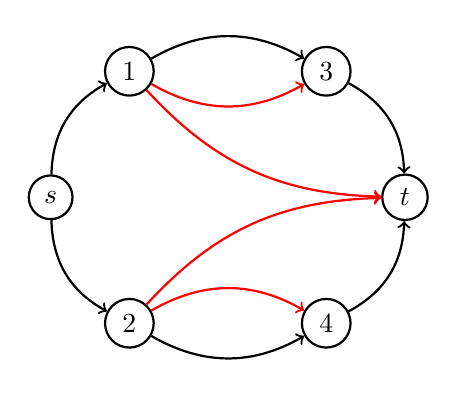
\begin{tikzpicture}[node distance={19mm}, thick , main/.style = {draw, circle}] 
    % Disegna i nodi del grafo
    \node[main] (0) {$s$};
    \node[main] (1) at (1, 1.6) {1};
    \node[main] (2) at (1, -1.6) {2};
    \node[main] (3) at (3.5, 1.6) {3};
    \node[main] (4) at (3.5, -1.6) {4};
    \node[main] (5) at (4.5, 0) {$t$};

    \draw[->] (0)[bend left] to (1);
    \draw[->] (0)[bend right] to (2);
    \draw[->] (1)[bend left] to (3);
    \draw[->] (2)[bend right] to (4);
    \draw[->] (4)[bend right] to (5);
    \draw[->] (3)[bend left] to (5);

    \draw[->] (1)[red, bend right] to (3);
    \draw[->] (2)[red, bend left] to (4);
    \draw[->] (2)[red, bend left = 23] to (5);
    \draw[->] (1)[red, bend right = 23] to (5);


\end{tikzpicture}
\end{tabular}\]

\begin{algo}{strongly compact network}{}
    Definiamo lo \textbf{Strongly compact} come $G^{sc} =(N^{sc}, E^{sc})$ originato dal network $G$:
    \begin{enumerate}
        \item Contrarre il grafo di tutti gli abundant cycles e degli archi esterni abbondanti.\\
        Sia $(r,S,T)$ l'input dopo la contrazione.
        \item Sia $N^{sc}\subseteq N(G)$ l'insieme dei nodi che sono adiacenti ad almeno un arco non abbondante.\\
        Ci riferiremo a $N(G)\setminus N^{sc}$ come l'insieme dei nodi \textit{strongly compactible}.
        \item Definiamo gli archi come $E^{sc} = E^1 \cup E^2$ dove:\\
        $E^1 = \{(i,j): i\in N^{sc}\land j\in N^{sc}\land (i,j)\in E(G)\}$\\
        $E^2 = \{(i,j): i\in N^{sc}\land j\in N^{sc}\land i\implies j\}$\\
        Dunque abbiamo archi originali in $E^1$ e pseudo archi che derivano dagli abundant path.
        
    \end{enumerate}
    
\end{algo}
    Il seguente algoritmo ha tempo $O(m + |E^{sc}|)$ in quanto si possono costruire gli pseudo archi in tempo $O(1)$ dato che viene dinamicamente preservata la chiusura transitiva. 
\begin{theo}{$f_{max} = f_{max}^{sc}$}{}
    Sia $f_{max}$ il flusso massimo nel network $G$ e sia $f_{max}^{sc}$ il flusso massimo in $G^{sc}$ allora 
    \[f_{max} = f_{max}^{sc}\]
\end{theo}
\begin{proof}
    Abbiamo già mostrato che qualsiasi flow in $G^{sc}$ può essere reindirizzato in $G$.
    Se invece prendiamo un flow in $G$, è possibile instradarlo in $G^{sc}$ usando la \textbf{flow decomposition} per ottenere da $f$ un insieme di path diversi almeno per un arco,
    \[f := \{P^0, P^1, ..., P^k\}\]
    Possiamo suddividere ancora ogni $P^a\in f$ in subpath \[P^{a}_{i\rightarrow j}| i\in N^{sc}\land j\in N^{sc}\land \forall q \in P^a_{i\rightarrow j}, q\not = i \land q\not = j \implies q\in N\setminus N^{sc}\] 
    A questo punto sostituiamo ogni $P^{a}_{i\rightarrow j}$ in $G$ non  interamente contenuto in $G^{sc}$ con lo pseudo arco corrispettivo $(i,j)$.
    \QED
\end{proof}



\section{Da sc-compact a $\Delta$-compact}
Il tempo $O(nm)$ si basa sul fatto che calcolare un max flow \textit{approssimato} su un grafo $\Delta$-compact sia di molto inferiore a calcolarlo sul grafo originale.

Prima di proseguire è importante distinguere diversi tipo di archi.
\begin{definition}{Classificazioni di capacità}{}
    Un arco $(i,j)$ rispetto a $\Delta$ ha:
    \begin{enumerate}
        \item \textbf{small capacity} se $r_{ij}+r_{ji} < \Delta/(64m^2)$
        \item \label{media}\textbf{medium capacity} se $r_{ij} \ge \Delta/(64m^2) \land r_{ij}+r_{ji} < 4\Delta$
        \item \begin{enumerate}
            \item \textbf{internal anti-abundant} se $r_{ij} \le 2\Delta \land r_{ji} \ge 2\Delta$
            \item \textbf{external anti-abundant} se non abundant 
        \end{enumerate}
        \item \textbf{abundant} se $r_{ij} \ge 2\Delta$
    \end{enumerate}
    
\end{definition}
Le Differenze tra strongly compact e $\Delta$-compact sono che:
\begin{enumerate}
    \item Nel $\Delta$-compact viene trasferita della capacità residua da alcuni archi ad altri o a pseudo archi creati appositamente per semplificare il grafo;
    \item Nel $\Delta$-compact i nodi adiacenti a archi con capacità residua troppo esigua vengono compattati.
\end{enumerate}

Un altro strumento necessario per decidere quali nodi compattare è la funzione \textit{potenziale}
\begin{definition}{Potential function}{}
    Dato un nodo $j\in N$ una funzione di capacità residua $r$ e un sottoinsieme di archi adiacenti a $j$ $\tilde{E}$  possiamo definire la funzione potenziale come: 
    \[\Phi (j, r, \tilde{E}) = \sum_{(i,j)\in \tilde{E}} r_{ij}-\sum_{(j,i)\in \tilde{E}} r_{ji}\] 
\end{definition}

Definiamo il set di archi \textbf{anti-abbondanti}, in un Network $G$, rispetto al parametro $\Delta$ come $A'(\Delta)$.
Nel seguente lemma utilizzeremo la funzione potenziale dove $\tilde{E} = A'(\Delta)$.
\begin{lemma}
    {}{}
    Sia $(S,T)$ un s-t cut in $G$ con $r(S,T)\le \Delta$, e sia $A' = A'(\Delta).$\\
    Supponiamo che esista $P\subseteq A'$ un path da $i\rightarrow j$ e che $(i,j)\in A'$. \\
    Se $r'$ è la nuova funzione di capacità residua ottenuta spostando $\delta$ unità di capacità residua da $P$ a $(i,j)$, allora possiamo affermare che:
    \begin{enumerate}
        \item $\forall k\in N(G),\ \Phi(k,r',A') = \Phi(k,r,A') $
        \item $r'(S,T) = r(S,T)$
    \end{enumerate}
\end{lemma}
    \begin{proof}
        \begin{enumerate}
            \item Il primo punto è intuitivo in quanto per ogni nodo in $P$ diverso da $i$ e $j$ sto sottraendo la stessa capacità residua sia in entrata che in uscita, mentre nei nodi $i$ e $j$ le sommatorie di $\Phi$ rimangono identiche.
            \item Il secondo punto è banale se $|P|= 1$ dunque consideriamo $|P|\ge 2$. Definiamo $P = p_1, ..., p_k$, $p_1 \in S$ e almeno un $p_q\in T$.\\
                Dato che abbiamo stabilito che $r(S,T) \le \Delta$ e che $P\subseteq A'$ ci troviamo sicuramente in una situazione di questo tipo:
                \[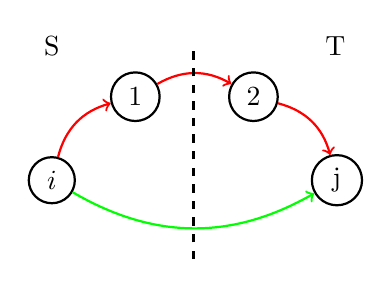
\begin{tikzpicture}[node distance={15mm}, thick , main/.style = {draw, circle}] 
                    % Disegna i nodi del grafo
                    \node[main] (0) {$i$};
                    \node[main] (1) [above right of = 0] {1};
                    \node[main] (2) [right of = 1] {2};
                    \node[main] (3) [below right of = 2] {j};
                    \node at (0,1.7) {S};
                    \node at (3.6,1.7) {T};

                    \draw[->] (0) [red, bend left] to (1);
                    \draw[->] (1) [red, bend left] to (2);
                    \draw[->] (2) [red, bend left] to (3);
                    \draw[->] (0) [green, bend right] to (3);

                    \draw[dashed] (1.8,-1) -- (1.8,1.7);
                \end{tikzpicture}\]
                In quanto se un arco di $P$ passasse da T a S violerebbe $r(S,T)\le \Delta$ dato che $\forall (a,b)\in A'(\Delta),\ r_{ab} > 2\Delta \land r_{ba}\ge 2\Delta$, avremmo che
                \[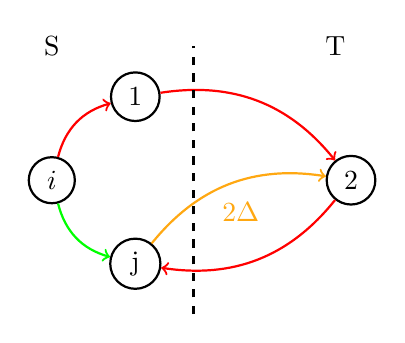
\begin{tikzpicture}[node distance={15mm}, thick , main/.style = {draw, circle}] 
                    % Disegna i nodi del grafo
                    \node[main] (0) {$i$};
                    \node[main] (1) [above right of = 0] {1};
                    \node[main] (2) at (3.8,0) {2};
                    \node[main] (3) [below right of = 0] {j};
                    \node at (0,1.7) {S};
                    \node at (3.6,1.7) {T};

                    \draw[->] (0) [red,bend left] to (1);
                    \draw[->] (1) [red,bend left] to (2);
                    \draw[->] (2) [red,bend left] to (3);
                    \draw[->] (3) [thick = 1.5, darktangerine, bend left] to (2);
                    \draw[->] (0) [green, bend right] to (3);

                    \draw[dashed] (1.8,-1.7) -- (1.8,1.7);
                    \node at (2.4, -.4) {\text{\color{darktangerine}{$2\Delta$}}};
                \end{tikzpicture}\]
            Una volta appurato ciò risulta evidente che il trasferimento di capacità residua non influenza la capacità residua del taglio. \QED
        \end{enumerate}
    \end{proof}
    \begin{definition}{$\Delta$-compactible}{}
        Un nodo j si dice $\Delta$-compactible se $|\Phi (j, r, A')| <\Delta/(16nm)$ e non ha archi adiacenti di \hyperref[media]{media capacità}.

        In oltre un nodo j si dice \textit{very $\Delta$-compactible} se ogni arco anti-abbondante incidete $j$ ha capacità residua $< \Delta/(16nm)$
    
    \end{definition}
    Per costruire il $\Delta$-compact network vengono iterativamente trasferite unità di capacità residue di vari path a pseudo archi. Abbiamo già visto che
    questi trasferimenti non influenzano il max-flow. I trasferimenti continuano finché tutti i nodi $\Delta$-compactible non diventano very $\Delta$-compactible.
    \begin{definition}
        {Transferrable residual capacity}{}
        Per poter trasferire $\delta$ capacità da un path $P$ da $i\rightarrow j$ all'arco $(i,j)$ è necessario che:
        \begin{enumerate}
            \item $|P|\ge 2$
            \item $r(P) > 0$
            \item $P\subseteq A'$
        \end{enumerate}
    \end{definition} 
    La capacità che viene trasferita da è $\delta = r(P) = \min_{(a,b)\in P} r(a,b)$, dunque ogni volta almeno un arco anti-abbondante viene saturato. 
    Se esiste un path $P\subseteq A'\ da\ i\rightarrow j $ ma $(i,j)\not \in E(G)$ allora viene creato come pseudo arco. 

    Alla fine tutti i nodi che non vengono compattati formeranno il $\Delta$-compact network.
    \begin{definition}{$\Delta$-critical}{}
        Se un nodo $j$ non è $\Delta$-compactible $\implies$ $j$ è $\Delta$-critical.
    \end{definition}
    Il $\Delta$-compact network è formato dai tutti e soli i nodi $\Delta$-critical.







\newpage
\begin{algo}{improve-approx-2}{}
    $01.\quad \Delta := r(S,T)$\\
    $02.\quad$ let c be the number of $\Delta$-critical nodes\\
    $03.\quad$\textbf{if} $c>m^{9/16}$ \textbf{then}: find a $\Delta/(4m)$-optimal flow on $G[r]$\\
    $04.\quad$\textbf{else, if} $m^{1/3}\le c<m^{9/16}$ \textbf{then}:\\
    $05.\qquad$ let $G'$ denote $\Delta$-compact network\\
    $06.\qquad$ find a $\Delta/(8m)$-optimal flow $x'$ on $G'$\\
    $07.\qquad$ transform the flow $x'$ into a $\Delta/(4m)$-optimal flow $x^*$ on $G[r]$\\
    $08.\quad$ \textbf{else, if} $c < m^{1/3}$ \textbf{then}: \\
    $09.\qquad$ choose  $\min \Gamma\ s.t\  |N(G^{(\Delta, \Gamma')})| < 2m^{1/3}$\\
    $10.\qquad$ let $G'$ denote $(\Delta, \Gamma')$-compact network\\
    $11.\qquad$ find an optimal flow $x'$ on $G'$\\
    $12.\qquad$ transform the flow $x'$ into a $\Gamma$-optimal flow $x^*$ on $G[r]$\\

            
    
    
\end{algo}


\newpage
\section{Dubbi}
    
\section{Sostituzioni}
Di seguito tutta la terinologia che fa riferimento all'articolo
\begin{center}
    Max flows in O(nm) time, or better\\
    James B. Orlin*\\
    Revised: July 25, 2012\\
\end{center}
con accanto la relativa sostituzione. La sostituzione del termine nel seguente articolo è stata effettuata per 
motivi di comprensibilità o affinità con la bibliografia di riferimento. Tutti i termini che non appaiono in questa
 sezionie coincidono con quelli utilizzati nell'articolo.\\
$\begin{array}{lcccl}
      &orlin&          &here& description\\\hline
    1.& A & \rightarrow &E& \text{L'insieme degli archi}\\
    2.& x & \rightarrow &f& \text{La funzione del flow}
\end{array}$

\chapter*{Bibliografia}
    Le fonti sull'algoritmo di Goldberg-Rao e su quello di Prim vengono dai seguenti articoli:
   \begin{enumerate}
    \item  Max flows in O(nm) time, or better, Revised: July 25, 2012, James B. Orlin*
    \item The Goldberg-Rao Algorithm for the Maximum Flow Problem, October 18 2006, Dávid Papp
   \end{enumerate}


\end{document}